% File example.tex
% Contact: simonnet@ecole.ensicaen.fr
%
% version 1.0 (July 24, 2009)
% version 1.1 (September 3, 2009)
% add using of the optional command: \secondauthoraddr

\documentclass[10pt,twocolumn]{article}

% ICPRS Template Preamble
% Defines custom commands for the ICPRS conference template

% Page geometry for ICPRS format (18cm x 24cm on A4)
\usepackage[a4paper,top=2.85cm,bottom=2.85cm,left=1.5cm,right=1.5cm,columnsep=0.4cm]{geometry}

\makeatletter

% Author and affiliation commands
\newcommand{\authorname}[1]{\gdef\@authorname{#1}}
\newcommand{\authoraddr}[1]{\gdef\@authoraddr{#1}}
\newcommand{\secondauthoraddr}[1]{\gdef\@secondauthoraddr{#1}}

% Keywords command
\newcommand{\keywords}{\noindent\textbf{Keywords:} }

% Abstract command (redefine existing command to match section format)
\renewcommand{\abstract}{\section*{Abstract}}

% Custom maketitle for ICPRS format (spans both columns)
\renewcommand{\maketitle}{%
  \twocolumn[{%
    \begin{center}
      {\Large\textbf{\@title}}\\[0.5em]
      {\large\textbf{\@authorname}}\\[0.3em]
      {\@authoraddr}\\
      \@ifundefined{@secondauthoraddr}{}{\@secondauthoraddr\\}
    \end{center}
    \vspace{1em}
  }]%
}

\makeatother 

%other package

% vectorial font
\usepackage{lmodern}

\usepackage{graphicx}
\usepackage{times}


\begin{document}
\noindent

% This should produce references in the order they appear
\bibliographystyle{ieeetr}

\title{Instructions for Preparing and Transferring Final Papers to \\ICPRS 2021}

\authorname{Anonymous}
\authoraddr{Do NOT include authors' names of affiliations}

\maketitle

\keywords
Maximum 5 keywords placed before the abstract.

\abstract
This is where the abstract should be placed. It should consist
of one paragraph and a concise summary of the material
discussed in the article below. It is preferable not to use
footnotes in the abstract, the title or indeed anywhere in the paper. The acknowledgement
for funding organisations etc. is placed in a separate section at
the end of the text. We wish you success with the preparation
of your manuscript.

\section{Introduction}
Papers for ICPRS-2021 need to be submitted for review by the \textbf{15 November 2020}. The submission should be the format described here and should be \textbf{anonymous}. If your paper is accepted, a final camera-ready non-anonymous version should be submitted, using the same electronic submission system, no later than the \textbf{29 January 2021}. Papers received after that date will not be included in the Proceedings. Your final version should be prepared taking into account the comments made by the reviewers and available to authors via the submission system. The Proceedings produced for ICPRS-2021 will contain \textbf{all} the papers accepted \textbf{and presented} in the conference.  

\section{Manuscript preparation}
Full papers must be typed in English. This instruction page is
an example of the format and font sizes to be used. MS Word
users can download from the conference site these
instructions in Word format. LaTeX is preferred as it is easier to change paper style and formatting.

These are detailed instructions valid for any word
processor. In the title of the paper the initial letters should be
capitalised in all words except articles and prepositions (e.g.:
in, a, an, and, the, there, their, do, on, of, from, with, at etc.).
E.g. "ErDoped Si Nanocrystals as a Candidate for Optical
Amplification" The type should be boldface 18pt and centred
on the page. The authors' names (in the final non-anonymous version) are typed in capital and lower
case bold letters and centred on the page. Directly under the
authors' names in capital and lower case letters and also
centred are the authors' affiliation(s), address(es), plus email
address(es) of (at least) the corresponding author. Manuscripts must be
typed single spaced using 10 point characters. Only Times,
Times Roman, Times New Roman and Symbol fonts are
accepted. The text must fall within a frame of 18 cm x 24 cm
centred on an A4 page (21 cm x 29.7 cm).Paragraphs are
separated by 6 points and with no indentation. The text of the
full papers is written in two columns and justified. Each
column has a width of 8.8 cm and the columns are separated
by a margin of 0.4 cm. The maximum length of the full paper
is 6 pages (min 4 pages). \textbf{Do not number the pages and avoid the use of footnotes}. The final format in
which the papers will appear on the Proceedings will be a
PDF file. Authors are required to upload a \textbf{PDF} file of their
final paper to be included directly in the Proceedings. \textbf{All
PDF files should NOT be locked and all fonts and
graphics should be embedded}.

\subsection{Figures and tables}
Figures and tables should be centred in the column, numbered
consecutively throughout the text, and each should have a
caption underneath it (see for example Table 1). Care should
be taken that the lettering is not too small. All figures and
tables should be included in the electronic versions of the full
paper. We cannot guarantee that any printed version of the
proceedings will use colour.


\begin{figure}[h]
\centering
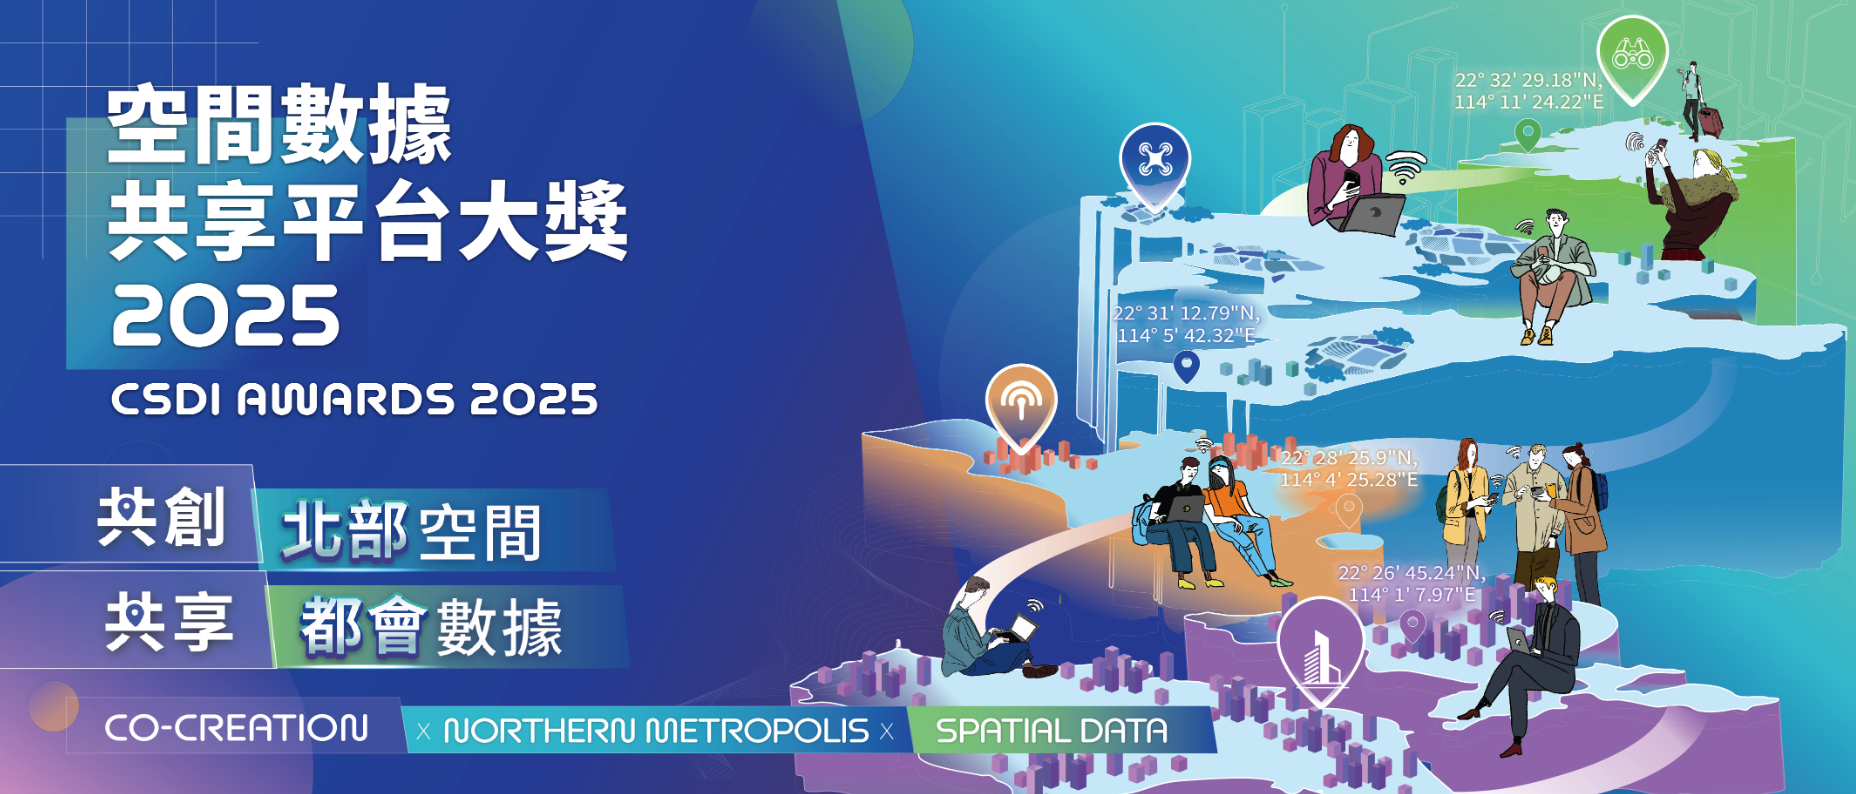
\includegraphics[width=0.4\textwidth]{figures/template_figure_1.png}
\caption{\label{tab1}This is an example of a figure caption.} 
\end{figure}



\subsection{Equations}
Equations should be typed within the text, centred, and should
be numbered consecutively throughout the text. They should
be referred to in the text as Equation (n). Their numbers
should be typed in parentheses, flush right, as in the following
example.
\begin{equation}
	    PA + A'P - PBR^{-1}B'P + Q  =  0 \enspace.
\end{equation}

\section{Generating a {PDF} file}
The PDF format will be the final format under which the
papers will appear in the Proceedings. Therefore you are
required to submit your paper as a PDF document. If this is not
possible, Postscript format is also accepted as long as no fonts
other than the recommended fonts are used.

You can use any of the popular free LaTeX editors (e.g. Kile, TexMaker, etc).

\section{Electronic submission of the full paper}
The submission process for ICPRS 2021 should be done on
line at http://www.icprs.org

A PDF version of your final paper is required. It should
be expected that after your submission, your paper is
published directly from the file you send without any further
proofreading. Therefore, it is advisable for the authors to
print a hard copy of their final version and read it carefully.

Note that the publisher reserves the right not to publish a paper that is deemed to be poorly formatted or with poor use of English.

\section{Your References}
The list of references should be ordered in the same order as
first cited in the text. All references should be cited in the
text, and using square brackets such as \cite{ref01} and \cite{ref01,ref02}. We
recommend the use of IEEE Transactions style for references. \textit{Avoid any references
that could identify any of the authors, e.g. avoid "as we showed in ..."}

\section*{Acknowledgements}
The acknowledgement for funding organisations etc. should
be placed in a separate section at the end of the text.



Thank you for your cooperation in complying with these
instructions.


\bibliography{IEEEabrv,references}


\end{document}
